\newif\ifrevtex
\revtextrue

\ifrevtex
    \documentclass[aps,final,twocolumn,letterpaper,nofootinbib]{revtex4-1}
\else
    \documentclass[twocolumn]{article}
\fi

%\usepackage[letterpaper,hmargin=0.8in,vmargin=0.8in]{geometry}
\usepackage{graphicx}

\usepackage{amsmath,amssymb}
\usepackage{siunitx}

\usepackage{cleveref}

%\usepackage{mathpazo}
\usepackage{microtype}

\usepackage{diagbox}
\usepackage{multirow}

\usepackage{color}
%\usepackage[printwatermark]{xwatermark}
%\newwatermark[allpages,color=red!10,angle=45,scale=3,xpos=0,ypos=0]{DRAFT}

\usepackage{tikz}

\newcommand\RR{\mathbb{R}}
\DeclareMathOperator\im{im}

\newcommand{\mb}{\mathbf}

%\usepackage{tikz}
%\usetikzlibrary{arrows}
%\usetikzlibrary{angles,patterns,calc}

\newcommand\headers{
    \title{Rigiditea: web-based rigidity algorithms}
    \author{Tony Zhang and Menghua Wu}
    \date{May 17, 2017}    
    \begin{abstract}
        We present Rigiditea,
        a native client-side web-based implementation of two algorithms
        for testing generic rigidity of graphs:
        the $n$-dimensional randomized infinitesimal-rigidity-based algorithm
        and the deterministic pebble game algorithm for two-dimensional rigidity.
        For the latter, we provide a step-by-step visualization of the algorithm
        for aid in understanding the algorithm.
    \end{abstract}
}


\ifrevtex\relax\else\headers\fi
\begin{document}
\ifrevtex\headers\fi

\maketitle



% % % % % % % % % %
%    INTRODUCTION
% % % % % % % % % %

\tableofcontents

\section{Introduction}

The theory of linkages TODO TODO TODO
finds obvious applications.
For example, 

We implemented two major algorithms for generic rigidity.
The first, which works in $n$ dimensions,
considers a random embedding of the graph into $\RR^n$
and computes the number of infinitesimal degrees of freedom (dof)
as described in \cite[\S4.4.2]{gfalop}.
Infinitesimal rigidity of the random embedding always implies generic rigidity;
the converse holds with high probability.

The second algorithm is the famous \emph{pebble game algorithm},
first introduced by Jacobs and Hendrickson in 1997~\cite{jacobs97}.
Briefly, it considers TODO TOOD

To the best of our knowledge,
there do not exist convenient implementations of
either rigidity algorithm.
In particular,
we were unable to find an sort of graphical interface
for the infinitesimal algorithm,
and only found a Java applet for the pebble game \cite{stjohnapplet}.


TODO TODO

Let us outline the remainder of this paper.
In \cref{sec:arch}, we describe the structure of our web application.
We next develop the theory behind the two rigidity algorithms
in \cref{sec:pebble,sec:infrigid}
to the level of detail necessary for understanding our work.
We conclude with a discussion of possible extensions to Rigiditea.

\section{Architecture}
\label{sec:arch}

blah blah blah

\subsection{Interface}

blah
 
\subsection{Backend}
blah

We provide an aesthetic interface
to design and analyze linkages as 2D planar graphs.

\begin{figure}[ht]
\begin{tikzpicture}
\node at (0,0) {
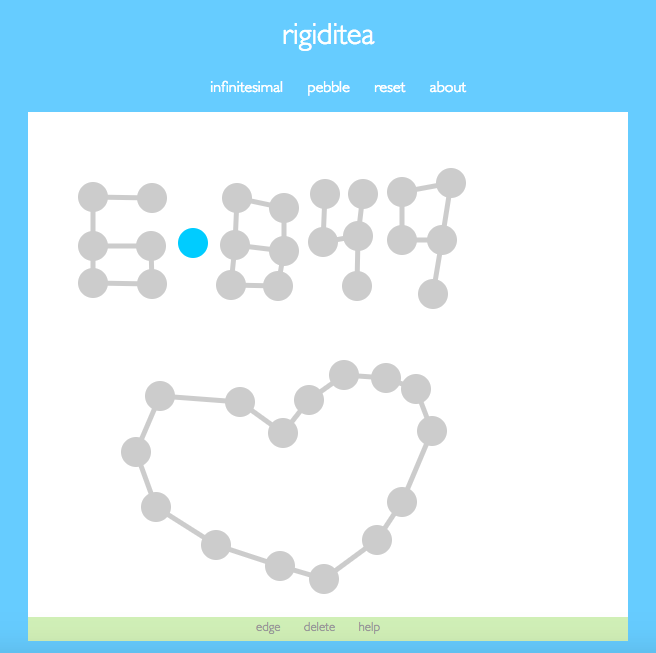
\includegraphics[scale=.3]{img/ui}
};
\draw (-3,-2.7) rectangle (3,2);
\node at (0,-1.5) {\large graph-drawing canvas};

\draw (-2,2.2) rectangle (2,2.7);
\node at (-2.5,2.45) {menu};

\draw (-1.5,-3) rectangle (1.5,-3.3);
\node at (-2.4,-3.15) {controls};
\end{tikzpicture}
\caption{High level overview of graphical user interface.
We aimed for a simple, but powerful design.}
\label{fig:ui}
\end{figure}

First, a user may click anywhere on the canvas to add a new node to the graph.
After creating nodes,
a user can control the user interface through one of two ways:
the menu bar and the control panel.
The former focuses on algorithm running and general information,
while the latter is tailored towards graph creation.
Figure \ref{fig:ui} points out these elements in the actual interface.
In addition to the menu and control panel,
we also provide keyboard shortcuts to streamline the user experience.
Table \ref{tab:menu} enumerates the various commands available,
their functionalities, and keyboard shortcuts.

\begin{table}[ht]
\caption{Menu items and descriptions}
\begin{tabular}{c | p{0.5\linewidth} | c}
item & description & shortcut \\ \hline
pebble & advances pebble algorithm one step
(one pebble exchange) & $\to$\\
reset & resets defaults, initializes new graph & r \\
about & background information about algorithms,
web application, and further reading & a \\
\end{tabular}
\label{tab:menu}
\end{table}

\begin{table}[ht]
\caption{Control panel items and descriptions}
\begin{tabular}{c c | p{0.5\linewidth} | c}
\multirow{3}{*}{menu} &
item & description & shortcut \\ \hline
edge & draws an edge between two selected vertices & e\\
delete & deletes all selected components, including incident edges
to selected nodes & x \\
help & provides information about graph designing interface,
including keyboard shortcuts & h \\
\end{tabular}
\label{tab:ctrl}
\end{table}

The GUI was created using \texttt{d3.js},
an open-source data visualization library for web applications.
We selected this library
to directly link graph data objects to SVG elements on the canvas.

\section{Pebble game visualization}
\label{sec:pebble}

blahbiy blah
\section{Infinitesimal rigidity}
\label{sec:infrigid}

The algorithm is straightforwardly presented in \cite[\S4.4.2]{gfalop},
so we provide a brief sketch.
Suppose we have a graph $G = (V, E)$ of $n$ vertices and $m$ edges.
Given a $d$-dimensional embedding of the vertices,
each edge provides a linear constraint
on the allowed infinitesimal motions of $V$.
In matrix form, we can write
\begin{equation}
    R\mb v = 0
\end{equation}
for a \emph{rigidity matrix}~$R$ of shape $dn \times m$
and an infinitesimal motion $\mb v \in \RR^{dn}$,
whose components are the $d$ components
of the infinitesimal motion of each of $n$ vertices.

The space of allowed infinitesimal motions is then $\ker R$.
However, some of these motions are trivial,
corresponding to the infinitesimal generators of rigid motions in $\RR^d$,
which form a $\binom{d+1}{2}$-dimensional vector space:
the Lie algebra $\mathfrak e(d)$ of the \emph{Euclidean group},
the isometry group of $\RR^d$.

Once we exclude these trivial motions,
we would naively expect the subspace of nontrivial infinitesimal motions
to have dimension
\begin{equation}
    \dim\ker R - \binom{d+1}{2} = dn - \dim\im R - \binom{d+1}{2},
\end{equation}
as presented in \cite{gfalop}.

This formula is generally correct,
but fails badly for some elementary examples.
For instance, take $K_2$, the graph of two vertices joined by an edge.
The rigidity matrix will have rank 1,
so for sufficiently large $d$,
we expect negative degrees of freedom:
\[
    dn - 1 - \binom{d+1}{2} < 0.
\]
Of course, $K_2$ should have no degrees of freedom for any~$d$.

Indeed, the naive analysis above
assumed that the subspace of trivial motions in $\ker R$
was $\binom{d+1}{2}$ dimensional:
that is, each nontrivial infinitesimal isometry of $\RR^d$
produced a nontrivial infintiesimal motion of our graph.
This assumption is generally false.
In our $K_2$ example,
if $d=3$, 
the infinitesimal generator
of the rotation about the single edge
produces the trivial infinitesimal motion 0
of the two vertices.


MORE PROFO MORE PROOF TODO 

\subsection{Correction to dof formula}

We present a correction to the  in \cite{gfalop}




%\section{Discussion}

\section{Extensions}

\begin{itemize}
    \item
    Undo feature
    \item
    Graph export into FOLD
    \item
    Visualize rigid components
    \item
    Extend to other pebble games like in \cite{lee08, chubynsky07}
\end{itemize}


\section*{Acknowledgements}


\bibliography{rigiditea}{}
\bibliographystyle{plain}






\end{document}

